\chapter{Problem Definition}\label{ch:problem-definition}
\section{Introduction}\label{sec:pd-intro}
The system we consider in this thesis is Interactive Myocontrol (section \ref{sec:interactivemyocontrol}), as we have seen in the relative section the input data of our machine learned controller comes from the eight sEMG sensors of the myobracelet and the output data are the activation levels of the nine DOFs of the prosthetic hand.
The problem we are going to study is what we call \textit{activation overshooting}: whenever a participant increase her muscle activation we expect that the prosthesis would in turn increase the applied force / torque; however, if we have a non-linear learning model like the one used in Interactive Myocontrol, this behaviour is not guaranteed. This kind of behaviour should be prevented and avoided by all means because can easily lead to potentially catastrophic failures: in practice whenever a participants increase her force in order to acquire, for example, a better grip on an object the results is the opposite to her expectation, e.g. the prosthesis drop the object.
Overshooting cannot be easily solved gathering more training data for the participant: this would require her to apply a large amount of force which could lead her to muscle strain, fatigue and frustration. Therefore we decided to study in the direction of "mechanically" amend the machine learning model in order to make it more reliable with respect to overshooting.
%
%
%
\section{Formal Definition}\label{sec:pd-formal-def}
In order to be able to amend the machine using an automated procedure we needed to define the overshooting problem in a strictly formal way: in the following we show how we arrived to the formal definition.
For sake of convenience we briefly consider a 2D-reduced exemplary S in which are contained the samples generated by three actions: rest, power grasp and wrist flexion. As can be seen in figure \ref{fig:heatmap} the training set can be seen as a set of clusters, each corresponding to a certain action.
\begin{figure}[ht]
    \centering
    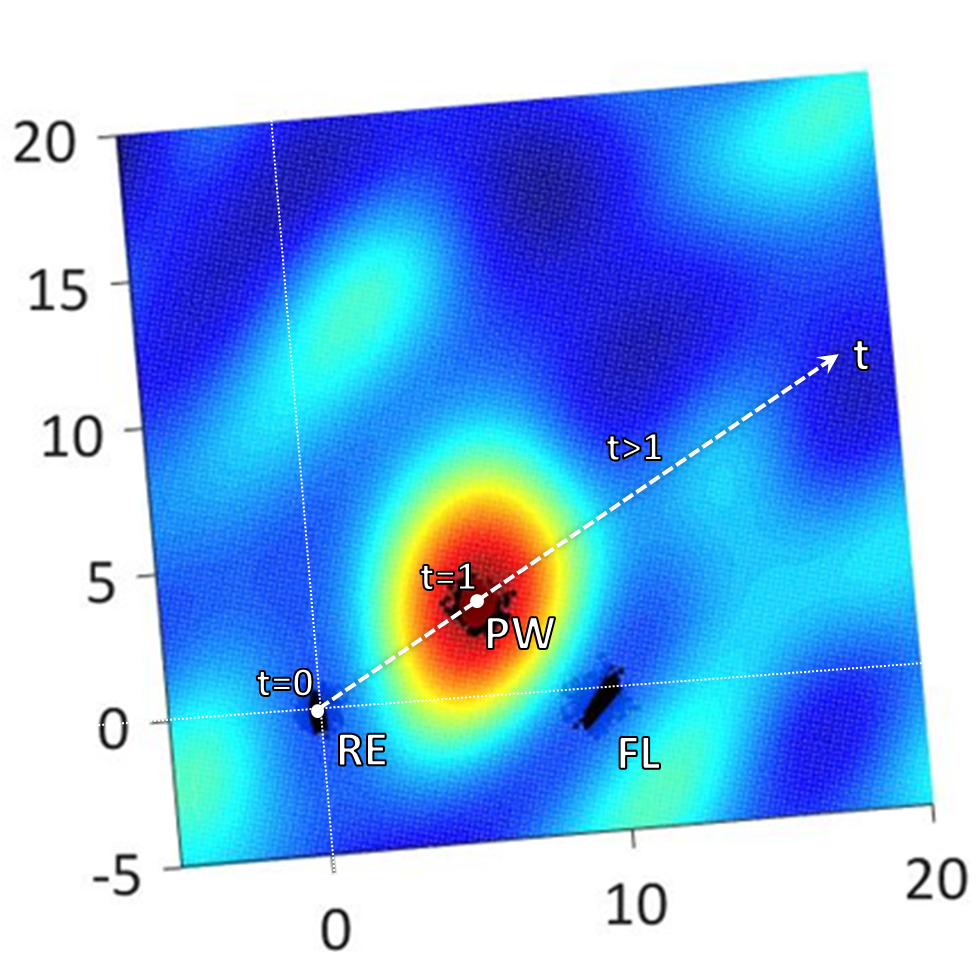
\includegraphics[width=0.8\textwidth]{Images/heatmap_DOF1.png}
    \caption{A 2D-reduced exemplary dataset S, obtained after gathering observations for three actions (black dots; rest, RE; power grasp, PW; wrist flexion, FL); the colour of the heat map denotes the value of the target value for power grasping, $f_{PW}$ . Values of the input space lying on the straight line $\overline{RE} + (\overline{PW} - \overline{RE})t_{PW}$ roughly denote power grasping with increasing strength.}
    \label{fig:heatmap}
\end{figure}
We define as $\overline{RE}$, $\overline{PW}$, $\overline{FL}$ the centers of the clusters corresponding respectively to the actions rest, power grasp and wrist flexion. In the figure is possible to see, as an heatmap, the function $f_{PW}$ obtained by training the learning model seen in section \ref{sec:ML} using the training set S.  
We decided to assume the straight line of the type $\overline{RE} + (\overline{PW} - \overline{RE})t_{PW}$ as the zone of the input space along which the participants signals move when she increase or decrease the force applied to a certain action; this assumption is justified by the physiology of the muscular activation and by our experimental observation.
As can be seen in figure \ref{fig:heatmap} between $t_{PW} = 0$ and $t_{PW} = 1$ the behaviour of the model is what we expected: the value of $f_{PW}$ increase with $t_{PW}$ and assume the maximum value for $t_{PW} = 1$, which corresponds to $\overline{PW}$. The problem become clear for the values of $t_{PW}$ greater than 1: almost immediately $f_{PW}$ begin to decrease and reaches 0 for $t_{PW} \approx 2$. In practice, the participant tries to apply more force and instead the hand open up, leading to drop the grasped object. This kind of failure is what we have called overshooting.
We are now able to give a formal definition of a model subject to overshooting:
\begin{equation}
    \exists a,t_a>1 : x = \overline{RE} + (\overline{a} - \overline{RE})t_{a} \implies f_a(x) < a_{max}
    \label{eq:overshooting}
\end{equation}
where $a$ indicates a general action on which we have trained the model and $a_{max}$ is the maximum activation value for that action. The other quantities correspond to what we have seen before but for a general action $a$.
Obviously the muscular activation in reality is not as precise and constant as we have supposed, therefore it will deviates from the straight line $\overline{RE} + (\overline{a} - \overline{RE})t_{a}$ and, as consequence, our definition of model subject to overshooting doesn't represent all the possible instances of overshooting. Nonetheless, thanks to the continuity of the nonlinear model we have chosen (RR-RFF sec. \ref{sec:ML}), the automated mending process manages to overall enhance the reliability of the system with respect to overshooting.
Overshooting can probably be defined in other ways, nevertheless we prefer to stick with the definition given in equation \ref{eq:overshooting} in order to limit as much as possible the subset of the input space we need to analyse to guarantee the absence of overshooting.
%
%
%
\section{Automated Procedure}
After having formally defined the overshooting problem we studied how to design an automated procedures which could bring the model to a state in which it wasn't subject to our definition of overshooting. In order to do so without changing drastically the structure of the learning model and of Interactive Myocontrol we decided to follow in the step of \cite{Strazzulla2017} and leverage the incrementality of the learning model used by Interactive Myocontrol.
The general idea of our automated procedure is to generate synthetic labelled samples which are then added to the original training set in order to modify the model and bring it in a state in which it is not subject to overshooting. With equation \ref{eq:overshooting} we have already given a preliminary definition of point in the input space which are affected by overshooting, it is reasonable to consider the above mentioned points as the one we are interested to add to the training set in order to modify the model so that they present the correct labels (e.g. they are no more subject to overshooting).
In order to preserve the coherence of the learning method we decided to keep the way we add points to the training set as similar as possible to the way the original training points are gathered: as seen before the training data are distributed in clusters corresponding to the different actions, therefore also our synthetic data will be distributed in the same way.
Given the characteristic of the training model and the possible interaction between the different actions, we decided to design our automated repair procedure as a iterative one:
\begin{enumerate}
    \item For each action of interest we search for an unsafe point (e.g. a point subject to overshooting, see equation \ref{eq:overshooting}), if no unsafe point is found for every action then the repair process is completed successfully.
    \item For each action for which we have found an unsafe point we generate a cluster centred on the point and we associate each point of the cluster with an appropriate label, then we add the point generated to the training set. We do nothing for the action for which we haven't found an unsafe point.
    \item The learning model is trained again but this time on the modified training set, then we continue with point 1.
\end{enumerate}
Obviously we still need to decide how to determine the appropriate label for the points we add to the training set: the natural choice appears to be the value $a_{max}$ seen in equation \ref{eq:overshooting} but experimentally we have found out that this kind of choice brings the repair procedure to need a longer time, and more unsafe points, in order to completely repair the model. This result is quite easy to understand: if our \textit{unsafety} condition is defined by equations \ref{eq:overshooting} we want that to every points $x = \overline{RE} + (\overline{a} - \overline{RE})t_{a}$ with $t_{a} >= 1$ corresponds a target value $f_a(x) >= a_{max}$ and if we consider the continuity of the learning model we have chosen, the adding of points with synthetic target value equals to $a_{max}$ it's unlikely to drastically modify the original model. Moreover from a theoretical point of view we would expect that to greater values of the input signals would correspond a greater activation level of the action. Therefore we chose as activation level for each synthetic point $x$ a value given by the following equation:
\begin{equation}
    y_{syn} = y_0 + c_a \cdot x_{proj}
    \label{eq:output_unsafe}
\end{equation}
where $c_a$ is the slope of the straight line connecting $(\overline{RE}, 0)$ and $(\overline{a}, a_{max})$ in the space $\mathbb{R}^9$ (e.g. remember that the input space is $\mathbb{R}^8$ and the activation value is a real number), $x_{proj}$ is the projection of the point $x$ on the straight line $\overline{RE} + (\overline{a} - \overline{RE})t_{a}$ and $y_0$ is a quantity we have determined experimentally.
